\chapter{控制理论}
\label{chap:control-theory}

第~\ref{chap:dynamical-systems-and-state-estimation}章研究了输入给定以后，状态怎样演化、扰动怎样传播，以及有限观测能够提供多少状态信息。第~\ref{chap:decision-theory-and-dynamic-risk}章又为跨时刻的行动后果建立了价值递推。还缺的一步是把输入本身变成待选择的对象：系统每到一个状态，都要依据当前可用信息决定下一次作用。这样形成的
\term{反馈}（feedback）会改变后续状态，后续状态又会改变未来的反馈。

这一步不能只靠写出一个优化目标。某个不稳定方向可能根本不受输入影响，某个影响决策的状态方向也可能无法从观测辨认；即使期望成本达到最小，轨迹仍可能穿过不可接受的区域。控制理论分别询问这些问题：哪些动态模式能够被输入改变，哪些模式能够被输出识别，怎样在长期稳定的前提下优化成本，以及怎样让每条允许轨迹都留在安全集合内。

本章先在线性状态空间中建立可控、可稳定、可观测和可检测四个结构条件。它们为线性二次调节和稳态滤波说明“解为什么存在且能稳定系统”。随后，我们从有限时域价值递推完整推出Riccati递推，并将成本最优与安全集合保持分开。最后把离散时间的Bellman原理缩到一个短时间区间，得到连续时间的Hamilton--Jacobi--Bellman方程。四节讨论的是同一个受控动态的不同要求；一个要求成立，不能替代其余要求。
\section{判断输入能否改变、观测能否区分动态模式}
\label{sec:control-feedback-structure}
\subsection{开环、状态反馈与输出反馈}
考虑离散时间线性时不变系统
\begin{equation}
  \begin{aligned}
    \bm{x}_{t+1}
      &=\bm{A}\bm{x}_t+\bm{B}\bm{u}_t,\\
    \bm{y}_t
      &=\bm{C}\bm{x}_t,
  \end{aligned}
  \label{eq:control-state-space}
\end{equation}
其中$\bm{x}_t\in\mathbb{R}^{n}$是状态，$\bm{u}_t\in\mathbb{R}^{m}$是控制输入，
$\bm{y}_t\in\mathbb{R}^{p}$是观测。矩阵维度相应为
$\bm{A}\in\mathbb{R}^{n\times n}$、$\bm{B}\in\mathbb{R}^{n\times m}$和
$\bm{C}\in\mathbb{R}^{p\times n}$。这里明确令直接传递矩阵为零，因此时刻$t$先由
$\bm{x}_t$产生$\bm{y}_t$，控制器再计算$\bm{u}_t$。若保留
$\bm{y}_t=\bm{C}\bm{x}_t+\bm{D}\bm{u}_t$并允许$\bm{u}_t$依赖当前
$\bm{y}_t$，两式会形成需要另行求解适定性的代数环；另一种无环约定是只让控制使用
截至$t-1$的观测。

“用当前状态计算动作”与“用当前读数计算动作”限制了控制器能使用的信息，不能仅靠
同一个反馈增益符号将两者混用。
\begin{definition}[开环控制与反馈控制]
\label{def:control-open-loop-state-output-feedback}
对式~\eqref{eq:control-state-space}，若$\bm{u}_0,\bm{u}_1,\bm{u}_2,\ldots$事先指定，
输入不根据运行中实际出现的状态修正，就称为\term{开环控制}（open-loop control）。
若状态能够直接取得，依据当前状态选择动作的
\[
  \bm{u}_t=\kappa_t(\bm{x}_t)
\]
是状态反馈；只有观测历史可用时，
\[
  \bm{u}_t
  =
  \mu_t(\bm{y}_0,\ldots,\bm{y}_t;
  \bm{u}_0,\ldots,\bm{u}_{t-1})
\]
称为输出反馈，其中空的初始控制历史按空序列处理。
\end{definition}
由于本节采用零直接传递，
当前观测$\bm{y}_t$不含尚未计算的$\bm{u}_t$。写出依赖真实状态的公式，不等于
传感器已经提供了该状态。

反馈把原系统与控制律合成一个新的闭环动力系统，因而还要重新检查解是否存在且唯一。离散时间递推只要每一步的反馈有定义，就能逐步生成轨迹；连续时间系统则通常要求动态与反馈满足局部Lipschitz等适定性条件。若反馈在切换面不连续，必须改用适合不连续右端的解概念，不能只凭形式上的闭环方程断言轨迹唯一。

最简单的线性状态反馈取
\begin{equation}
  \bm{u}_t=-\bm{K}\bm{x}_t,
  \qquad
  \bm{x}_{t+1}
  =(\bm{A}-\bm{B}\bm{K})\bm{x}_t.
  \label{eq:control-state-feedback}
\end{equation}
因此闭环离散系统渐近稳定，当且仅当$\bm{A}-\bm{B}\bm{K}$的全部特征值都严格位于单位圆内。这里的负号只是约定；若写$\bm{u}_t=\bm{F}\bm{x}_t$，对应闭环矩阵就是$\bm{A}+\bm{B}\bm{F}$。

反馈能否把不稳定特征值移入单位圆，取决于输入是否真正作用到相应状态方向。这不是优化算法精度问题，而是矩阵对$(\bm{A},\bm{B})$本身的结构性质。
\subsection{可达子空间与可控性}
把式~\eqref{eq:control-state-space}连续展开$N$步，可得
\begin{equation}
  \bm{x}_N
  =
  \bm{A}^{N}\bm{x}_0
  +
  \sum_{t=0}^{N-1}
  \bm{A}^{N-1-t}\bm{B}\bm{u}_t.
  \label{eq:control-reachability-unrolling}
\end{equation}
固定初态后，终态中能被控制改变的部分属于
\[
  \operatorname{span}
  \{\bm{B},\bm{A}\bm{B},\ldots,
    \bm{A}^{N-1}\bm{B}\}
\]
的列空间。这些列依次表示一次输入经过零步、一步直至$N-1$步传播后能够产生的状态方向。
\begin{definition}[可控性]
\label{def:control-controllability}
若对任意初态$\bm{x}_0$和任意目标状态$\bm{x}_{\mathrm f}$，都存在有限时刻$N$及输入序列$\bm{u}_0,\ldots,\bm{u}_{N-1}$，使$\bm{x}_N=\bm{x}_{\mathrm f}$，则称$(\bm{A},\bm{B})$可控。
\end{definition}
对线性时不变系统，“从任意初态到任意终态”与“从零到任意终态”等价：式~\eqref{eq:control-reachability-unrolling}对输入线性，自由响应$\bm{A}^N\bm{x}_0$可以移到目标一侧。这两种性质都蕴含任意初态可以在有限时间驱动到零，但反向一般不成立。后一种较弱的性质称为\term{零可控性}。例如，标量系统$A=0,B=0$会使任意初态在一步后自然变为零，却无法从零到达非零状态；当$\bm{A}$可逆时，零可控性才可反推出这里定义的可控性。
\begin{theorem}[Kalman可控性秩判据]
\label{thm:control-controllability-rank}
定义可控性矩阵
\begin{equation}
  \mathcal{C}(\bm{A},\bm{B})
  =
  \begin{bmatrix}
    \bm{B}&\bm{A}\bm{B}&\cdots&\bm{A}^{n-1}\bm{B}
  \end{bmatrix}.
  \label{eq:control-controllability-matrix}
\end{equation}
系统$(\bm{A},\bm{B})$可控，当且仅当
\[
  \operatorname{rank}\mathcal{C}(\bm{A},\bm{B})=n.
\]
\end{theorem}
\begin{proof}
先取$N=n$。把输入按逆时间顺序堆成向量，式~\eqref{eq:control-reachability-unrolling}中的受控部分可以写成
\[
  \mathcal{C}(\bm{A},\bm{B})
  \begin{bmatrix}
    \bm{u}_{n-1}\\
    \bm{u}_{n-2}\\
    \vdots\\
    \bm{u}_0
  \end{bmatrix}.
\]
若可控性矩阵满行秩，它的列张成$\mathbb{R}^n$，所以对任意$\bm{x}_{\mathrm f}-\bm{A}^n\bm{x}_0$都能找到输入，系统可控。

反过来，若该矩阵秩小于$n$，其列空间是$\mathbb{R}^n$的真子空间。Cayley--Hamilton定理说明$\bm{A}^n$可写成$\bm{I},\bm{A},\ldots,\bm{A}^{n-1}$的线性组合；继续乘$\bm{A}$可知，每个$\bm{A}^k\bm{B}$（$k\geq n$）仍落在$\mathcal{C}(\bm{A},\bm{B})$的列空间中。延长时域不会增加新的可达方向，因而从零出发无法到达该列空间外的状态，系统不可控。
\end{proof}
最小的算例是标量积分系统$x_{t+1}=x_t+u_t$。给定$x_0$与目标$x_{\mathrm f}$，一步取$u_0=x_{\mathrm f}-x_0$即可到达，因而其可控性矩阵$[1]$满秩。若改成二维系统
\[
  \bm{A}=
  \begin{bmatrix}
    1&1\\
    0&1
  \end{bmatrix},
  \qquad
  \bm{B}=
  \begin{bmatrix}
    0\\1
  \end{bmatrix},
\]
则当前输入先改变第二个坐标，经过一次状态传播后再影响第一个坐标。此时
\[
  \begin{bmatrix}\bm{B}&\bm{A}\bm{B}\end{bmatrix}
  =
  \begin{bmatrix}
    0&1\\
    1&1
  \end{bmatrix}
\]
满秩，两个坐标都可达。相反，若$\bm{A}=\bm{I}$而$\bm{B}=(1,0)^{\top}$，输入无论作用多久都只能改变第一个坐标；延长时域不会补出缺失方向。

图~\ref{fig:control-reachable-directions}保留刚才的二维系统，并为教学示意暂时加入
$|u_0|,|u_1|\leq1$。从零出发，一步只能沿$\bm B$移动，两步终态为
$\bm x_2=\bm A\bm B u_0+\bm B u_1=(u_0,u_0+u_1)^\top$。
有界输入形成一个平行四边形；解除幅值限制后，两个独立方向张成整个平面，
这才对应秩判据中的无约束可控性。图中可达区域的面积与能到达任意状态是不同说法。
\begin{figure}[htbp]
  \centering
  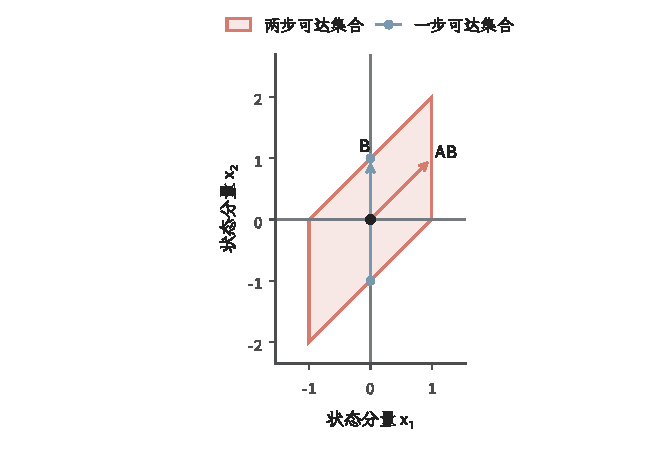
\includegraphics[width=\linewidth]{figures/math-preparation/concept-revision-dynamics/reachable-directions.pdf}
  \caption{教学系统$\bm A=\left[\begin{smallmatrix}1&1\\0&1\end{smallmatrix}\right]$、
  $\bm B=(0,1)^\top$与零初态。蓝色线段为$|u_0|\leq1$时的一步可达集合，
  红色区域为$|u_0|,|u_1|\leq1$时的两步可达集合；箭头标出$\bm B$与$\bm A\bm B$。
  输入先改变第二个坐标，经一次状态传播后获得新的方向。输入幅值界只服务于有限区域的绘图，
  不属于定理~\ref{thm:control-controllability-rank}的无约束假设。}
  \label{fig:control-reachable-directions}
\end{figure}

连续时间线性系统$\dot{\bm{x}}=\bm{A}\bm{x}+\bm{B}\bm{u}$具有相同问题，但输入通过积分累积。由状态转移公式，
\[
  \bm{x}(T)
  =
  e^{\bm{A}T}\bm{x}_0
  +
  \int_0^T e^{\bm{A}(T-s)}\bm{B}\bm{u}(s)\,\mathrm{d}s.
\]
定义时域$T>0$上的\term{可控Gram矩阵}
\begin{equation}
  \bm{W}_{\mathrm c}(T)
  =
  \int_0^T
  e^{\bm{A}s}\bm{B}\bm{B}^{\top}e^{\bm{A}^{\top}s}
  \,\mathrm{d}s.
  \label{eq:control-controllability-gramian}
\end{equation}
连续线性系统在$[0,T]$上可控，当且仅当$\bm{W}_{\mathrm c}(T)\succ\bm{0}$。事实上，对任意$\bm{q}\in\mathbb{R}^n$，
\[
  \bm{q}^{\top}\bm{W}_{\mathrm c}(T)\bm{q}
  =
  \int_0^T
  \lVert
    \bm{B}^{\top}e^{\bm{A}^{\top}s}\bm{q}
  \rVert_2^2\,\mathrm{d}s.
\]
若Gram矩阵奇异，就存在非零$\bm{q}$使被积函数恒为零，该方向与所有受控终态增量正交，因而不可达。若Gram矩阵正定，则对所需增量$\bm{d}=\bm{x}_{\mathrm f}-e^{\bm{A}T}\bm{x}_0$取
\[
  \bm{u}(s)
  =
  \bm{B}^{\top}e^{\bm{A}^{\top}(T-s)}
  \bm{W}_{\mathrm c}(T)^{-1}\bm{d},
\]
代入状态转移公式便得到终态增量$\bm{d}$。这个Gram判据依赖线性时不变结构；一般非线性系统即使在一点把Jacobian矩阵代入，也只能得到局部线性化信息，不能据此推出全局可控。

秩判据回答“整个状态空间是否可达”，但有时我们只需判断某个动态模式是否受控。在复数域上考察$\bm{A}$的左特征向量会得到更直接的判据。
\begin{theorem}[Popov--Belevitch--Hautus（PBH）可控性判据]
\label{thm:control-pbh-controllability}
矩阵对$(\bm{A},\bm{B})$可控，当且仅当对$\bm{A}$的每个复特征值$\lambda$都有
\begin{equation}
  \operatorname{rank}
  \begin{bmatrix}
    \lambda\bm{I}-\bm{A}&\bm{B}
  \end{bmatrix}
  =n.
  \label{eq:control-pbh-controllability}
\end{equation}
等价地，不存在非零左特征向量$\bm{q}^{\ast}$满足$\bm{q}^{\ast}\bm{A}=\lambda\bm{q}^{\ast}$且$\bm{q}^{\ast}\bm{B}=\bm{0}$。
\end{theorem}
\begin{proof}
若存在这样的$\bm{q}$，则对每个$k\geq0$，
\[
  \bm{q}^{\ast}\bm{A}^k\bm{B}
  =
  \lambda^k\bm{q}^{\ast}\bm{B}
  =\bm{0}.
\]
所以可控性矩阵的每一列都位于$\bm{q}^{\ast}$的零空间，不可能满行秩。

反向可用$\bm{A}$不变子空间说明。若可控性矩阵不满秩，它的列空间$\mathcal{R}$是一个真子空间，并且$\bm{A}\mathcal{R}\subseteq\mathcal{R}$。于是正交补$\mathcal{R}^{\perp}$在$\bm{A}^{\ast}$下不变。复数域上的非零有限维不变子空间包含$\bm{A}^{\ast}$的一个特征向量$\bm{q}$。它正交于$\mathcal{R}$，特别有$\bm{q}^{\ast}\bm{B}=\bm{0}$，从而式~\eqref{eq:control-pbh-controllability}在相应特征值处不满秩。
\end{proof}
\subsection{可控分解与可稳定性}
完全可控时，极点配置定理允许通过状态反馈配置闭环特征值；稳定系统并不总需要这么强的条件。若某个不可控模式本身已经衰减，就没有必要通过输入移动它。
\begin{definition}[可稳定性]
\label{def:control-stabilizability}
若存在矩阵$\bm{K}$，使$\bm{A}-\bm{B}\bm{K}$的全部特征值严格位于单位圆内，则称离散时间矩阵对$(\bm{A},\bm{B})$可稳定。
\end{definition}

这个结论可以由Kalman可控分解看清。令$\mathcal{R}$为可控性矩阵的列空间，并选择以$\mathcal{R}$的一组基为前若干列的可逆矩阵$\bm{T}$。由于$\bm{A}\mathcal{R}\subseteq\mathcal{R}$且$\operatorname{col}(\bm{B})\subseteq\mathcal{R}$，在坐标$\bm{z}=\bm{T}^{-1}\bm{x}$下有
\[
  \bm{T}^{-1}\bm{A}\bm{T}
  =
  \begin{bmatrix}
    \bm{A}_{\mathrm c}&\bm{A}_{12}\\
    \bm{0}&\bm{A}_{\mathrm{uc}}
  \end{bmatrix},
  \qquad
  \bm{T}^{-1}\bm{B}
  =
  \begin{bmatrix}
    \bm{B}_{\mathrm c}\\
    \bm{0}
  \end{bmatrix},
\]
其中$(\bm{A}_{\mathrm c},\bm{B}_{\mathrm c})$可控。把$\bm{K}\bm{T}$分块写成
$[\bm{K}_{\mathrm c}\ \bm{K}_{\mathrm{uc}}]$后，闭环矩阵在同一坐标下变为
\[
  \begin{bmatrix}
    \bm{A}_{\mathrm c}-\bm{B}_{\mathrm c}\bm{K}_{\mathrm c}
    &
    \bm{A}_{12}-\bm{B}_{\mathrm c}\bm{K}_{\mathrm{uc}}\\
    \bm{0}&\bm{A}_{\mathrm{uc}}
  \end{bmatrix}.
\]
反馈可以通过$\bm{K}_{\mathrm c}$配置可控块的特征值，却不能改变不可控块$\bm{A}_{\mathrm{uc}}$的特征值。因此，存在稳定化反馈当且仅当不可控块本身稳定。PBH矩阵在特征值$\lambda$处不满秩，恰好表示$\lambda$属于这个不可控块；所以只需排除不稳定和临界的不可控模式：
\begin{equation}
  \operatorname{rank}
  \begin{bmatrix}
    \lambda\bm{I}-\bm{A}&\bm{B}
  \end{bmatrix}
  =n
  \quad
  \text{对每个满足 }|\lambda|\geq1
  \text{ 的 }\lambda\in\sigma(\bm{A}).
  \label{eq:control-pbh-stabilizability}
\end{equation}
可控必然推出可稳定，反向并不成立。这个差别在无限时域调节中很重要：已经稳定但无法控制的模式可以留在原处，无法控制的不稳定模式却会使任何线性反馈都失败。
\begin{example}[不可控但可稳定的系统]
\label{ex:control-stabilizable-not-controllable}
令
\[
  \bm{A}=
  \begin{bmatrix}
    1.2&0\\
    0&0.5
  \end{bmatrix},
  \qquad
  \bm{B}=
  \begin{bmatrix}
    1\\0
  \end{bmatrix}.
\]
可控性矩阵
\[
  \begin{bmatrix}\bm{B}&\bm{A}\bm{B}\end{bmatrix}
  =
  \begin{bmatrix}
    1&1.2\\
    0&0
  \end{bmatrix}
\]
只有秩$1$，第二个模式不可控。但它的特征值为$0.5$，已经位于单位圆内。取$\bm{K}=(1,0)$，闭环特征值变成$0.2$和$0.5$，所以该系统可稳定。若交换$\bm{B}$的两个分量，使输入只能作用到$0.5$模式，则$1.2$模式不可控，系统便不可稳定。
\end{example}
\subsection{可观测性、可检测性与观测器}
控制器若只能看见输出，就要先问不同初态能否由输出序列区分。暂取输入为零；已知输入对输出的贡献可以计算并扣除，不改变以下结构判据。连续观察$n$个时刻得到
\begin{equation}
  \begin{bmatrix}
    \bm{y}_0\\
    \bm{y}_1\\
    \vdots\\
    \bm{y}_{n-1}
  \end{bmatrix}
  =
  \underbrace{
  \begin{bmatrix}
    \bm{C}\\
    \bm{C}\bm{A}\\
    \vdots\\
    \bm{C}\bm{A}^{n-1}
  \end{bmatrix}}_{\mathcal{O}(\bm{C},\bm{A})}
  \bm{x}_0.
  \label{eq:control-observability-matrix}
\end{equation}
\begin{definition}[可观测性与可检测性]
\label{def:control-observability-detectability}
若式~\eqref{eq:control-observability-matrix}中的观测矩阵$\mathcal{O}(\bm{C},\bm{A})$满列秩，则称$(\bm{C},\bm{A})$可观测。若存在矩阵$\bm{L}$使$\bm{A}-\bm{L}\bm{C}$的全部特征值严格位于单位圆内，则称$(\bm{C},\bm{A})$可检测。
\end{definition}
可观测意味着有限输出序列能够唯一确定任意初态。这个秩条件也可以从“输出能否区分两个初态”直接证明。若$\mathcal{O}$满列秩，则线性方程~\eqref{eq:control-observability-matrix}至多有一个$\bm{x}_0$，所以输出序列唯一确定初态。反之，若$\mathcal{O}$不满列秩，就存在非零$\bm{v}$满足$\mathcal{O}\bm{v}=\bm{0}$；初态$\bm{x}_0$与$\bm{x}_0+\bm{v}$在前$n$个时刻产生相同输出。Cayley--Hamilton定理又使所有$\bm{C}\bm{A}^k\bm{v}$（$k\geq n$）都是前$n$项的线性组合，所以继续观察也无法区分这两个初态。

可检测只要求所有无法从输出辨认的模式自行稳定；不可见但会衰减的状态不会阻止估计误差趋于零。二者的PBH判据分别为
\begin{align}
  \operatorname{rank}
  \begin{bmatrix}
    \lambda\bm{I}-\bm{A}\\
    \bm{C}
  \end{bmatrix}
  &=n
  &&\text{对每个 }\lambda\in\sigma(\bm{A}),
  \label{eq:control-pbh-observability}\\
  \operatorname{rank}
  \begin{bmatrix}
    \lambda\bm{I}-\bm{A}\\
    \bm{C}
  \end{bmatrix}
  &=n
  &&\text{对每个 }|\lambda|\geq1.
  \label{eq:control-pbh-detectability}
\end{align}
把$\bm{A}$换成$\bm{A}^{\top}$、把$\bm{B}$换成$\bm{C}^{\top}$，可控性矩阵的转置正是观测矩阵。对偶矩阵对$(\bm{A}^{\top},\bm{C}^{\top})$应用上述Kalman分解，可知反馈无法移动它的不可控块，而该块正对应原系统的不可观测模式。又因为
\[
  \bm{A}^{\top}-\bm{C}^{\top}\bm{L}^{\top}
  =
  (\bm{A}-\bm{L}\bm{C})^{\top},
\]
两侧具有相同特征值，所以式~\eqref{eq:control-pbh-detectability}既是必要条件也是充分条件：不可观测块稳定时，可以配置其余观测器误差模式；不可观测块含危险特征值时，任何$\bm{L}$都无法消除它。这就是可控与可观测、可稳定与可检测之间的线性代数对偶。

连续时间版本只改变“危险模式”的稳定区域。对$\dot{\bm{x}}=\bm{A}\bm{x}+\bm{B}\bm{u}$，可稳定性要求
\[
  \operatorname{rank}
  \begin{bmatrix}
    \lambda\bm{I}-\bm{A}&\bm{B}
  \end{bmatrix}
  =n
  \quad
  \text{对每个满足 }\operatorname{Re}\lambda\geq0
  \text{ 的 }\lambda\in\sigma(\bm{A});
\]
对输出$\bm{y}=\bm{C}\bm{x}$，可检测性要求相应的纵向PBH矩阵满列秩。分解与对偶论证和离散情形相同，只把单位圆外替换为闭右半平面。该接口将在连续时间Riccati稳态条件中使用。

继续使用示例~\ref{ex:control-stabilizable-not-controllable}中的$\bm{A}$。若$\bm{C}=(1,0)$，不稳定的$1.2$模式可以观测，稳定的$0.5$模式不可观测；系统不可观测但可检测。若改成$\bm{C}=(0,1)$，输出完全看不到$1.2$模式，估计误差中的该分量会增长，系统不可检测。
表~\ref{tab:control-structural-properties}把输入与输出两侧放在同一尺度下比较。
“完整恢复或到达”要求每个方向都可处理；“只求长期稳定”允许遗漏那些本来就会衰减的
方向。前者更强，却未必是当前控制目标必需的条件。

\begin{table*}[htbp]
  \centering
  \begin{tabularx}{\linewidth}{lXXX}
    \toprule
    性质 & 所比较的对象 & 哪些方向必须处理 & 二维例的判断\\
    \midrule
    可控 & 输入与终态 & 全部状态方向 & 否，输入无法改变第二坐标\\
    可稳定 & 反馈与闭环谱 & 不稳定及临界模式 & 是，$1.2$模式受控\\
    可观测 & 初态与输出序列 & 全部状态方向 & 否，输出不含第二坐标\\
    可检测 & 观测器与误差谱 & 不稳定及临界模式 & 是，$1.2$模式可见\\
    \bottomrule
  \end{tabularx}
  \caption{线性系统的四种结构条件。二维教学例固定
  $\bm A=\operatorname{diag}(1.2,0.5)$、$\bm B=(1,0)^\top$、$\bm C=(1,0)$。
  第二模式虽不可控且不可观测，却自行衰减；若将其特征值改为$1.1$，可稳定与可检测
  两项也会失败。连续时间用特征值实部代替模长判断危险模式。}
  \label{tab:control-structural-properties}
  \label{tab:control-structural-comparison}
\end{table*}

\subsection{观测器与状态反馈的谱分离}
状态不可直接取得时，可以用\term{Luenberger观测器}根据模型、输入和输出更新估计：
\begin{equation}
  \widehat{\bm{x}}_{t+1}
  =
  \bm{A}\widehat{\bm{x}}_t+\bm{B}\bm{u}_t
  +
  \bm{L}\bigl(
    \bm{y}_t-\bm{C}\widehat{\bm{x}}_t
  \bigr).
  \label{eq:control-luenberger-observer}
\end{equation}
令估计误差$\bm{e}_t=\bm{x}_t-\widehat{\bm{x}}_t$，直接相减得到
\[
  \bm{e}_{t+1}
  =
  (\bm{A}-\bm{L}\bm{C})\bm{e}_t.
\]
因此可检测性正是选择$\bm{L}$使误差渐近消失所需的结构条件。

将状态反馈改为$\bm{u}_t=-\bm{K}\widehat{\bm{x}}_t$后，用$\bm{x}_t$和$\bm{e}_t$作为联合状态可得
\begin{equation}
  \begin{bmatrix}
    \bm{x}_{t+1}\\
    \bm{e}_{t+1}
  \end{bmatrix}
  =
  \begin{bmatrix}
    \bm{A}-\bm{B}\bm{K}&\bm{B}\bm{K}\\
    \bm{0}&\bm{A}-\bm{L}\bm{C}
  \end{bmatrix}
  \begin{bmatrix}
    \bm{x}_t\\
    \bm{e}_t
  \end{bmatrix}.
  \label{eq:control-separation-block}
\end{equation}
该矩阵是分块上三角矩阵，其特征值是两个对角块特征值的并集。因此，只要$(\bm{A},\bm{B})$可稳定且$(\bm{C},\bm{A})$可检测，就能分别选择$\bm{K}$和$\bm{L}$，使整个确定性线性闭环稳定。这一
\term{分离原理}并不表示估计与控制在所有问题中都互不影响；非线性、约束、模型误差
或风险敏感目标可能破坏这种简单分离。
表~\ref{tab:control-structural-properties}中的输入和输出两侧由转置联系。
完全结构条件覆盖全部状态方向，稳定化结构条件只排除危险的遗漏方向；
后面的Riccati条件会分别调用这两侧的较弱条件，而不会要求每个系统都完全可控且完全可观测。

\section{在二次成本下设计反馈与估计器}
\label{sec:control-lqr-riccati}

结构分析已经说明哪些方向可受控、哪些方向可观测。现在在这些条件下给定二次成本，
寻找具体反馈。有限时域的Bellman递推保持价值函数的二次形式，因而导出Riccati递推；
无限时域还需稳定化条件，不能把有限时域可配方直接当作稳态解存在的证明。
\subsection{二次价值函数与有限时域Riccati递推}
结构条件说明稳定反馈是否可能存在，却没有选择具体反馈。现在为状态偏离和控制用力分别计价。
\begin{definition}[有限时域线性二次调节]
\label{def:control-finite-horizon-lqr}
考虑有限时域随机线性系统
\begin{equation}
  \bm{x}_{t+1}
  =
  \bm{A}\bm{x}_t+\bm{B}\bm{u}_t+\bm{w}_t,
  \qquad t=0,\ldots,T-1,
  \label{eq:control-lqr-dynamics}
\end{equation}
以及成本
\begin{equation}
  J
  =
  \mathbb{E}\left[
    \bm{x}_T^{\top}\bm{Q}_T\bm{x}_T
    +
    \sum_{t=0}^{T-1}
    \left(
      \bm{x}_t^{\top}\bm{Q}\bm{x}_t
      +
      \bm{u}_t^{\top}\bm{R}\bm{u}_t
    \right)
  \right].
  \label{eq:control-lqr-cost}
\end{equation}
这里$\bm{Q},\bm{Q}_T\in\mathbb{R}^{n\times n}$且$\bm{Q},\bm{Q}_T\succeq\bm{0}$，$\bm{R}\in\mathbb{R}^{m\times m}$且$\bm{R}\succ\bm{0}$。半正定状态代价允许某些状态方向不直接计价；正定控制代价保证每一步关于$\bm{u}_t$的二次目标严格凸。

在可用信息规定的非预见控制策略中最小化$J$，称为\term{线性二次调节}
（linear-quadratic regulation, LQR）。
\end{definition}

先假设状态完全可见，且$\bm{w}_t$相互独立、均值为零、协方差为$\bm{\Sigma}_{\mathrm{w}}$，并与当前状态和动作独立。令$\mathcal{F}_t=\sigma(\bm{x}_0,\ldots,\bm{x}_t)$表示截至时刻$t$可用的状态信息，并用$\Pi_t$表示从$t$到$T-1$的允许反馈策略；对任意$\pi\in\Pi_t$，控制$\bm{u}_{\tau}$必须对$\mathcal{F}_{\tau}$可测，不能预先利用未来噪声。定义从时刻$t$起的最优剩余成本
\[
  V_t(\bm{x})
  =
  \inf_{\pi\in\Pi_t}
  \mathbb{E}\left[
    \bm{x}_T^{\top}\bm{Q}_T\bm{x}_T
    +
    \sum_{\tau=t}^{T-1}
    \bigl(
      \bm{x}_{\tau}^{\top}\bm{Q}\bm{x}_{\tau}
      +
      \bm{u}_{\tau}^{\top}\bm{R}\bm{u}_{\tau}
    \bigr)
    \,\middle|\,\bm{x}_t=\bm{x}
  \right].
\]
这里的下确界对适应当前状态信息的策略取，而不是对事先固定的开环控制序列取。终端价值为
$V_T(\bm{x})=\bm{x}^{\top}\bm{Q}_T\bm{x}$\scite{math-anderson2007lqr}
第~\ref{chap:decision-theory-and-dynamic-risk}章的Bellman原理给出
\begin{equation}
  V_t(\bm{x})
  =
  \min_{\bm{u}}
  \left\{
    \bm{x}^{\top}\bm{Q}\bm{x}
    +
    \bm{u}^{\top}\bm{R}\bm{u}
    +
    \mathbb{E}
    \left[
      V_{t+1}(
        \bm{A}\bm{x}+\bm{B}\bm{u}+\bm{w}_t)
    \right]
  \right\}.
  \label{eq:control-lqr-bellman}
\end{equation}
\begin{theorem}[有限时域LQR与Riccati递推]
\label{thm:control-finite-horizon-lqr}
在上述条件下，最优价值具有形式
\[
  V_t(\bm{x})
  =
  \bm{x}^{\top}\bm{P}_t\bm{x}+c_t,
\]
其中$\bm{P}_T=\bm{Q}_T$、$c_T=0$。令
\begin{equation}
  \begin{aligned}
    \bm{S}_t
      &=
      \bm{R}+\bm{B}^{\top}\bm{P}_{t+1}\bm{B},\\
    \bm{K}_t
      &=
      \bm{S}_t^{-1}
      \bm{B}^{\top}\bm{P}_{t+1}\bm{A}.
  \end{aligned}
  \label{eq:control-lqr-gain}
\end{equation}
则最优控制为
\[
  \bm{u}_t^{\ast}=-\bm{K}_t\bm{x}_t,
\]
而$\bm{P}_t$满足离散Riccati递推
\begin{equation}
  \bm{P}_t
  =
  \bm{Q}
  +
  \bm{A}^{\top}\bm{P}_{t+1}\bm{A}
  -
  \bm{A}^{\top}\bm{P}_{t+1}\bm{B}
  \bm{S}_t^{-1}
  \bm{B}^{\top}\bm{P}_{t+1}\bm{A}.
  \label{eq:control-discrete-riccati-recursion}
\end{equation}
噪声只进入常数项
\begin{equation}
  c_t
  =
  c_{t+1}
  +
  \operatorname{tr}(\bm{P}_{t+1}\bm{\Sigma}_{\mathrm{w}}).
  \label{eq:control-lqr-noise-constant}
\end{equation}
\end{theorem}
\begin{proof}
采用反向归纳。终端时刻的结论由$\bm{P}_T=\bm{Q}_T,c_T=0$成立。假设$t+1$时刻价值已经具有所述形式。记
\[
  \bm{z}
  =
  \bm{A}\bm{x}+\bm{B}\bm{u}.
\]
零均值和独立性给出
\begin{align*}
  \mathbb{E}
  [V_{t+1}(\bm{z}+\bm{w}_t)]
  &=
  \mathbb{E}
  [(\bm{z}+\bm{w}_t)^{\top}
    \bm{P}_{t+1}
    (\bm{z}+\bm{w}_t)]
  +c_{t+1}\\
  &=
  \bm{z}^{\top}\bm{P}_{t+1}\bm{z}
  +
  \operatorname{tr}(\bm{P}_{t+1}\bm{\Sigma}_{\mathrm{w}})
  +c_{t+1}.
\end{align*}
交叉项的条件期望为零。将$\bm{z}$展开，并只收集与控制有关的项，Bellman目标成为
\begin{align*}
  &\bm{x}^{\top}
  (\bm{Q}+\bm{A}^{\top}\bm{P}_{t+1}\bm{A})
  \bm{x}
  +
  2\bm{u}^{\top}
  \bm{B}^{\top}\bm{P}_{t+1}\bm{A}\bm{x}\\
  &\quad+
  \bm{u}^{\top}
  (\bm{R}+\bm{B}^{\top}\bm{P}_{t+1}\bm{B})
  \bm{u}
  +
  \operatorname{tr}(\bm{P}_{t+1}\bm{\Sigma}_{\mathrm{w}})
  +c_{t+1}.
\end{align*}
因为$\bm{R}\succ\bm{0}$且$\bm{P}_{t+1}\succeq\bm{0}$，$\bm{S}_t\succ\bm{0}$。以式~\eqref{eq:control-lqr-gain}中的$\bm{K}_t$配方，
\begin{align*}
  &\bm{u}^{\top}\bm{S}_t\bm{u}
  +
  2\bm{u}^{\top}
  \bm{B}^{\top}\bm{P}_{t+1}\bm{A}\bm{x}\\
  &\quad=
  (\bm{u}+\bm{K}_t\bm{x})^{\top}
  \bm{S}_t
  (\bm{u}+\bm{K}_t\bm{x})
  -
  \bm{x}^{\top}\bm{K}_t^{\top}
  \bm{S}_t\bm{K}_t\bm{x}.
\end{align*}
第一项非负，并且仅在$\bm{u}=-\bm{K}_t\bm{x}$时为零。把剩余二次项合并，恰好得到式~\eqref{eq:control-discrete-riccati-recursion}；与状态无关的项给出式~\eqref{eq:control-lqr-noise-constant}。Riccati右端保持半正定，于是归纳可以继续到$t=0$。
\end{proof}
该证明同时解释了“二次价值族在Bellman备份下封闭”的含义：线性动态把状态与动作送入二次型，最小化动作后仍留下状态的二次型。一般非线性动态或非二次代价不具有这个闭合关系，不能仅把矩阵换成Jacobian矩阵就得到精确LQR。

噪声不改变反馈增益也有明确边界。这里用到了噪声条件均值为零、与当前决策独立，以及风险中性期望成本。若噪声均值非零，价值函数一般还需要线性项，最优控制会出现仿射偏置；若噪声分布受动作影响、与状态相关，或目标惩罚尾部风险，噪声可能直接改变反馈律。
\subsection{标量LQR的配方与反馈增益}
取无噪声标量系统
\[
  x_{t+1}=1.2x_t+u_t,
  \qquad
  Q=R=1.
\]
若下一步价值系数为$P_{t+1}$，则
\[
  S_t=1+P_{t+1},
  \qquad
  K_t=\frac{1.2P_{t+1}}{1+P_{t+1}},
\]
并且
\[
  P_t
  =
  1+1.44P_{t+1}
  -
  \frac{1.44P_{t+1}^2}{1+P_{t+1}}
  =
  1+\frac{1.44P_{t+1}}{1+P_{t+1}}.
\]
当终端代价$P_T=0$时，倒数第一步有$P_{T-1}=1$，$K_{T-1}=0$；最后一个动作之后没有状态代价，所以此时不用力。再向前一步得到$P_{T-2}=1.72$和$K_{T-2}=0.6$。时域变长后，远离终端的增益逐渐接近稳态值。
\subsection{无限时域LQR与稳定化Riccati解}
本小节切换到确定性系统，即在式~\eqref{eq:control-lqr-dynamics}中令$\bm{w}_t=\bm{0}$。对时不变、无折扣的无限时域问题，考虑总成本
\[
  J_{\infty}
  =
  \sum_{t=0}^{\infty}
  \left(
    \bm{x}_t^{\top}\bm{Q}\bm{x}_t
    +
    \bm{u}_t^{\top}\bm{R}\bm{u}_t
  \right).
\]
该级数并非对任意控制都有限；稳定化条件用于保证最优反馈下的状态和控制充分衰减。希望$\bm{P}_t$和$\bm{K}_t$不再随时间变化。将$\bm{P}_{t+1}=\bm{P}_t=\bm{P}$代入式~\eqref{eq:control-discrete-riccati-recursion}，得到
\term{离散代数Riccati方程}（discrete algebraic Riccati equation, DARE）：
\begin{equation}
  \bm{P}
  =
  \bm{Q}
  +
  \bm{A}^{\top}\bm{P}\bm{A}
  -
  \bm{A}^{\top}\bm{P}\bm{B}
  (\bm{R}+\bm{B}^{\top}\bm{P}\bm{B})^{-1}
  \bm{B}^{\top}\bm{P}\bm{A}.
  \label{eq:control-dare}
\end{equation}
一个满足代数等式的矩阵未必就是所需解。控制所需的是
\term{稳定化解}：除满足$\bm{P}\succeq\bm{0}$外，它产生的
\[
  \bm{K}
  =
  (\bm{R}+\bm{B}^{\top}\bm{P}\bm{B})^{-1}
  \bm{B}^{\top}\bm{P}\bm{A}
\]
还要使$\bm{A}-\bm{B}\bm{K}$稳定。
\begin{theorem}[无限时域LQR的稳定化解]
\label{thm:control-infinite-horizon-lqr}
设$\bm{Q}\succeq\bm{0}$、$\bm{R}\succ\bm{0}$。若$(\bm{A},\bm{B})$可稳定，且$(\bm{Q}^{1/2},\bm{A})$可检测，则式~\eqref{eq:control-dare}存在唯一的半正定稳定化解$\bm{P}$。由该解得到的线性反馈使闭环渐近稳定，并给出无限时域二次成本的最优值$V(\bm{x})=\bm{x}^{\top}\bm{P}\bm{x}$。
\end{theorem}
\begin{proof}
这里给出决定条件作用的证明主线。对终端矩阵取$\bm{P}_N=\bm{0}$，从长度$N$的有限时域问题反向递推，并记初始时刻矩阵为$\bm{P}^{(N)}$。增加一个非负阶段成本不会降低最优成本，所以
\[
  \bm{0}\preceq
  \bm{P}^{(N)}
  \preceq
  \bm{P}^{(N+1)}.
\]
可稳定性保证存在某个$\overline{\bm{K}}$使$\bm{A}-\bm{B}\overline{\bm{K}}$稳定。始终采用这一反馈所得无限时域成本有限，因此它为所有有限时域最优成本提供统一二次上界。单调且有上界的半正定矩阵序列收敛到某个$\bm{P}\succeq\bm{0}$。Riccati映射连续，取极限便得到式~\eqref{eq:control-dare}。

令$\bm{A}_{\bm{K}}=\bm{A}-\bm{B}\bm{K}$。将DARE按最优增益重写为
\begin{equation}
  \bm{P}
  -
  \bm{A}_{\bm{K}}^{\top}
  \bm{P}\bm{A}_{\bm{K}}
  =
  \bm{Q}+\bm{K}^{\top}\bm{R}\bm{K}.
  \label{eq:control-dare-lyapunov}
\end{equation}
右侧半正定。现在用可检测性排除闭环中的非衰减模式。若
$\bm{A}_{\bm K}$存在特征对
$\bm{A}_{\bm K}\bm{z}=\lambda\bm{z}$，其中
$\bm{z}\neq\bm{0}$且$|\lambda|\geq1$，在
式~\eqref{eq:control-dare-lyapunov}两侧左乘$\bm{z}^{*}$、右乘$\bm{z}$，得到
\[
  (1-|\lambda|^2)\bm{z}^{*}\bm{P}\bm{z}
  =
  \lVert\bm{Q}^{1/2}\bm{z}\rVert_2^2
  +
  \lVert\bm{R}^{1/2}\bm{K}\bm{z}\rVert_2^2.
\]
左侧非正而右侧非负，所以两侧只能同时为零。特别地，
$\bm{Q}^{1/2}\bm{z}=\bm{0}$且$\bm{K}\bm{z}=\bm{0}$。于是
\[
  \bm{A}\bm{z}
  =
  (\bm{A}_{\bm K}+\bm{B}\bm{K})\bm{z}
  =
  \lambda\bm{z},
\]
这给出了$(\bm{Q}^{1/2},\bm{A})$无法检测的危险特征向量，与假设矛盾。因此
$\bm{A}_{\bm K}$的全部特征值严格位于单位圆内，极限解确实是稳定化解。

记$\bm{S}=\bm{R}+\bm{B}^{\top}\bm{P}\bm{B}$。对任意控制序列，把Bellman配方恒等式
沿前$N$步求和，得到
\[
  \sum_{t=0}^{N-1}
  \left(
    \bm{x}_t^{\top}\bm{Q}\bm{x}_t
    +
    \bm{u}_t^{\top}\bm{R}\bm{u}_t
  \right)
  +
  \bm{x}_N^{\top}\bm{P}\bm{x}_N
  =
  \bm{x}_0^{\top}\bm{P}\bm{x}_0
  +
  \sum_{t=0}^{N-1}
  (\bm{u}_t+\bm{K}\bm{x}_t)^{\top}
  \bm{S}
  (\bm{u}_t+\bm{K}\bm{x}_t).
\]
这里不能在令$N\to\infty$时直接丢掉终端项。若某个允许控制的总成本有限，则
\[
  \bm{Q}^{1/2}\bm{x}_t\to\bm{0},
  \qquad
  \bm{u}_t\to\bm{0};
\]
第二个结论使用了$\bm{R}\succ\bm{0}$。由
$(\bm{Q}^{1/2},\bm{A})$可检测，可选$\bm{L}$使
$\bm{A}-\bm{L}\bm{Q}^{1/2}$稳定，并把状态递推写成
\[
  \bm{x}_{t+1}
  =
  (\bm{A}-\bm{L}\bm{Q}^{1/2})\bm{x}_t
  +
  \bm{B}\bm{u}_t
  +
  \bm{L}\bm{Q}^{1/2}\bm{x}_t.
\]
右侧稳定线性系统的输入趋于零，因此$\bm{x}_t\to\bm{0}$，进而
$\bm{x}_N^{\top}\bm{P}\bm{x}_N\to0$。这就是可检测性在终端项论证中的具体作用。
总成本无限的控制自然不可能优于稳定反馈。令$N\to\infty$后，任意有限成本控制的成本
等于$\bm{x}_0^{\top}\bm{P}\bm{x}_0$加上一串
\[
  (\bm{u}_t+\bm{K}\bm{x}_t)^{\top}
  (\bm{R}+\bm{B}^{\top}\bm{P}\bm{B})
  (\bm{u}_t+\bm{K}\bm{x}_t)
\]
的极限和。采用$\bm{u}_t=-\bm{K}\bm{x}_t$时这些平方项为零，闭环稳定也使终端项趋零，故该反馈达到下界并最优。同一恒等式应用于两个半正定稳定化解，可知二者都表示同一最优成本，因而相等。
\end{proof}
示例中的标量DARE为
\[
  P=1+\frac{1.44P}{1+P},
  \qquad
  P^2-1.44P-1=0.
\]
半正定解是
\[
  P=\frac{1.44+\sqrt{6.0736}}{2}\approx1.952,
  \qquad
  K=\frac{1.2P}{1+P}\approx0.794.
\]
闭环系数$1.2-K\approx0.406$，位于单位圆内。另一个代数根为负，不表示非负无限时域成本，也不是这里的稳定化解。

可检测条件中的“输出”是$\bm{Q}^{1/2}\bm{x}$，不是传感器输出$\bm{C}\bm{x}$。它要求任何不被状态成本惩罚的不稳定模式都不存在。传感器的可检测性则决定估计误差能否稳定，两种条件服务于不同对象。

一个标量反例说明为何代数解和成本最优都不足以替代“稳定化”。令$A=1.2$、$B=1$、$Q=0$、$R=1$。系统可控，却因为$Q^{1/2}=0$而无法检测不稳定模式。DARE同时有$P=0$和$P=0.44$两个半正定解：前者给出$K=0$和不稳定闭环$1.2$，后者给出稳定闭环$1.2-1.2P/(1+P)=5/6$。然而原目标只惩罚控制，取$u_t=0$便以零成本达到全局最小；稳定化解对应正控制成本，反而不是该退化目标的最优解。可检测性正是用来排除这种“不稳定状态完全免费”的情形，不能在求出某个DARE根以后省略。

无限时域切换到确定性系统也不是无关紧要的简化。若每一步都有非零独立加性噪声，即使闭环稳定，状态协方差通常也会收敛到非零稳态值，单步期望状态成本便不会趋于零；无折扣累计期望成本因而通常发散。此时应明确改用长期平均成本、折扣成本或有限时域目标。只有当噪声及其传播方向恰好不被成本计入等退化情形，才可能避开这一结论。
\subsection{滤波Riccati对偶与LQG分离}
第~\ref{chap:dynamical-systems-and-state-estimation}章的有限时域Kalman滤波在每一步先传播协方差，再用新观测修正。若采用预测协方差$\bm{\Pi}_t$，状态噪声协方差为$\bm{\Sigma}_{\mathrm{w}}\succeq\bm{0}$，观测噪声协方差为$\bm{\Sigma}_{\mathrm{v}}\succ\bm{0}$，稳态预测方程可写成
\begin{equation}
  \bm{\Pi}
  =
  \bm{A}\bm{\Pi}\bm{A}^{\top}
  +\bm{\Sigma}_{\mathrm{w}}
  -
  \bm{A}\bm{\Pi}\bm{C}^{\top}
  (\bm{C}\bm{\Pi}\bm{C}^{\top}+\bm{\Sigma}_{\mathrm{v}})^{-1}
  \bm{C}\bm{\Pi}\bm{A}^{\top}.
  \label{eq:control-filter-dare}
\end{equation}
这里$\bm{\Pi}$是观测$\bm{y}_t$到来之前的预测误差协方差。令
\[
  \widehat{\bm{x}}_{t|t-1}
  =
  \mathbb{E}[\bm{x}_t\mid\mathcal{Y}_{t-1}],
\]
其中$\mathcal{Y}_{t-1}$包含截至$t-1$的观测和已执行控制，并在稳态记
\[
  \bm{\Pi}
  =
  \mathbb{E}\left[
    (\bm{x}_t-\widehat{\bm{x}}_{t|t-1})
    (\bm{x}_t-\widehat{\bm{x}}_{t|t-1})^{\top}
  \right].
\]
采用观测模型$\bm{y}_t=\bm{C}\bm{x}_t+\bm{v}_t$时，与式~\eqref{eq:control-filter-dare}口径一致的合并观测更新与一步预测为
\[
  \widehat{\bm{x}}_{t+1|t}
  =
  \bm{A}\widehat{\bm{x}}_{t|t-1}
  +\bm{B}\bm{u}_t
  +\bm{L}
  \bigl(
    \bm{y}_t-\bm{C}\widehat{\bm{x}}_{t|t-1}
  \bigr),
\]
其中
\[
  \bm{L}
  =
  \bm{A}\bm{\Pi}\bm{C}^{\top}
  (\bm{C}\bm{\Pi}\bm{C}^{\top}+\bm{\Sigma}_{\mathrm{v}})^{-1}.
\]
因此齐次预测误差矩阵是$\bm{A}-\bm{L}\bm{C}$。若把
$\bm{\Pi}\bm{C}^{\top}
(\bm{C}\bm{\Pi}\bm{C}^{\top}+\bm{\Sigma}_{\mathrm{v}})^{-1}$
称为观测更新增益，则从更新后估计传播到下一时刻时还要左乘$\bm{A}$；两种增益不能在同一协方差口径下混用。

将控制DARE中的
\[
  \bm{A}\leftrightarrow\bm{A}^{\top},
  \quad
  \bm{B}\leftrightarrow\bm{C}^{\top},
  \quad
  \bm{Q}\leftrightarrow\bm{\Sigma}_{\mathrm{w}},
  \quad
  \bm{R}\leftrightarrow\bm{\Sigma}_{\mathrm{v}},
\]
便得到这一形式。控制增益用输入压低状态成本，滤波增益用观测压低估计误差协方差；公式对偶不表示两者的随机变量含义相同。

一个常用的充分条件是$(\bm{C},\bm{A})$可检测、$(\bm{A},\bm{\Sigma}_{\mathrm{w}}^{1/2})$可稳定且$\bm{\Sigma}_{\mathrm{v}}\succ\bm{0}$。在这些条件及标准独立噪声假设下，协方差递推收敛到唯一稳定化半正定解，稳态滤波增益使估计误差动态稳定。可检测性保证危险状态模式能从观测纠正；过程噪声对偶条件排除Riccati方程在不稳定方向上的退化。有限时域滤波本身不要求协方差已经收敛，稳态公式也不能在系统时变、噪声统计变化或模型严重错设时直接替代逐时递推。

滤波结果怎样进入控制，还需要一条信息接口。在线性动态、二次成本、高斯初值与独立加性高斯噪声的标准有限时域设定中，令
\[
  \widehat{\bm{x}}_t
  =
  \mathbb{E}[\bm{x}_t\mid\mathcal{Y}_t],
  \qquad
  \bm{e}_t=\bm{x}_t-\widehat{\bm{x}}_t,
\]
其中$\mathcal{Y}_t$包含截至$t$的观测和已执行控制。条件期望的投影性质给出
\[
  \mathbb{E}[\bm{e}_t\mid\mathcal{Y}_t]=\bm{0},
  \qquad
  \mathbb{E}
  [\widehat{\bm{x}}_t^{\top}\bm{Q}\bm{e}_t]=0.
\]
因此条件状态成本分解为估计均值的二次成本与误差协方差项；在该设定下，Kalman误差协方差递推又不依赖所选控制值。Bellman递推中与当前动作有关的部分遂与完全状态LQR相同，只需把真实状态换成条件均值：
\[
  \bm{u}_t^{\ast}
  =
  -\bm{K}_t\widehat{\bm{x}}_t.
\]
这就是线性二次高斯控制中的\term{分离原则}：Kalman滤波器按估计误差设计，LQR增益按行动成本设计，再通过估计均值连接。它比前文确定性观测器的谱分离多给出期望成本最优性，但依赖噪声、信息和二次目标的特殊结构；受控观测噪声、风险敏感目标、输入或状态约束都可能使估计价值依赖未来控制，从而破坏这一分离。
\section{把轨迹安全转化为可行动作约束}
\label{sec:control-safety-cbf}

成本最优并不自动保证所有状态约束成立。本节另加轨迹必须留在安全集合内的要求，
用集合边界上的可行方向建立屏障条件，再把名义控制投影到可行输入集合。
这项保证与LQR成本是两种要求：安全条件先确定允许哪些动作，优化再从中选择。
\subsection{安全集合与正向不变性}
LQR惩罚偏离和控制强度，所得反馈对给定二次目标最优。但有限代价或渐近稳定都不保证状态从未越过危险区域。一个制动系统最终回到零速度，仍可能在停止前越过边界；一个平均成本很小的随机系统，也可能存在少量不可接受轨迹。安全控制需要逐轨迹描述允许状态，并证明闭环向量场不会把状态推出该集合。

离散系统可以先用一步条件看清这一要求。设闭环映射为$\bm{x}_{t+1}=F_{\kappa}(\bm{x}_t)$，安全集合为$S$。若
\begin{equation}
  F_{\kappa}(S)\subseteq S,
  \label{eq:control-discrete-invariance}
\end{equation}
则从$\bm{x}_0\in S$出发，归纳可得$\bm{x}_1\in S$，继而$\bm{x}_2\in S$，并对每个$t\geq0$都有$\bm{x}_t\in S$。反过来，若要求$S$中的每个初态都正向不变，取任意$\bm{x}\in S$考察第一步，就必须有$F_{\kappa}(\bm{x})\in S$。因此式~\eqref{eq:control-discrete-invariance}对确定性离散闭环既充分又必要。

例如，对$x_{t+1}=x_t+u_t$取安全集合$S=[0,\infty)$。反馈$u_t=-1.5x_t$产生$x_{t+1}=-0.5x_t$，状态幅值会趋于零，却从任意$x_0>0$在第一步就越过安全边界；反馈$u_t=-0.5x_t$则产生$x_{t+1}=0.5x_t$，既渐近稳定又保持非负。原系统能够到达负半轴只说明它可达，不能说明所选闭环应该到达那里。这个例子把可达、稳定与安全分成了三个不同判断。

连续时间不能只检查采样时刻的一步映射，因为轨迹可能在两个采样点之间越界。考虑控制仿射系统
\begin{equation}
  \dot{\bm{x}}
  =
  \bm{f}(\bm{x})+\bm{G}(\bm{x})\bm{u},
  \qquad
  \bm{u}\in U,
  \label{eq:control-affine-system}
\end{equation}
其中$\bm{x}\in\mathbb{R}^n$，$\bm{u}\in\mathbb{R}^m$，$\bm{G}(\bm{x})\in\mathbb{R}^{n\times m}$。假设$\bm{f}$和$\bm{G}$局部Lipschitz，所选反馈使闭环解存在且唯一。用连续可微函数$h:\mathbb{R}^n\to\mathbb{R}$定义安全集合
\begin{equation}
  S
  =
  \{\bm{x}:h(\bm{x})\geq0\}.
  \label{eq:control-safe-set}
\end{equation}
这里把定义~\ref{def:dynamical-invariant-limit-sets}中的正向不变性用于已经选定反馈的闭环系统。
\begin{definition}[正向不变集]
\label{def:control-forward-invariance}
若从任意$\bm{x}_0\in S$出发，闭环解在其存在的全部未来时刻都满足$\bm{x}(t)\in S$，则称$S$对该闭环系统正向不变。
\end{definition}
当边界$\partial S=\{\bm{x}:h(\bm{x})=0\}$光滑且$\nabla h(\bm{x})\neq\bm{0}$时，集合内侧对应$h$增大的方向。Nagumo切锥条件在这里化为：边界上的闭环速度必须指向集合内部或与边界相切，
\begin{equation}
  \dot h(\bm{x})
  =
  \nabla h(\bm{x})^{\top}
  \bigl(
    \bm{f}(\bm{x})+\bm{G}(\bm{x})\bm{u}
  \bigr)
  \geq0
  \quad
  \text{当 }h(\bm{x})=0.
  \label{eq:control-nagumo-boundary}
\end{equation}
只在边界检查这个条件适合理论判定，但控制器还需要在接近边界时提前限制动作。
图~\ref{fig:control-stability-safety}显示前述离散例。两条轨迹都趋近原点，但红色轨迹
在第一步进入负半轴，已违反安全要求。安全性约束的是整个运动过程，渐近稳定性约束的是
长期行为；只画最终状态会把这一区别隐藏掉。

\begin{figure}[htbp]
  \centering
  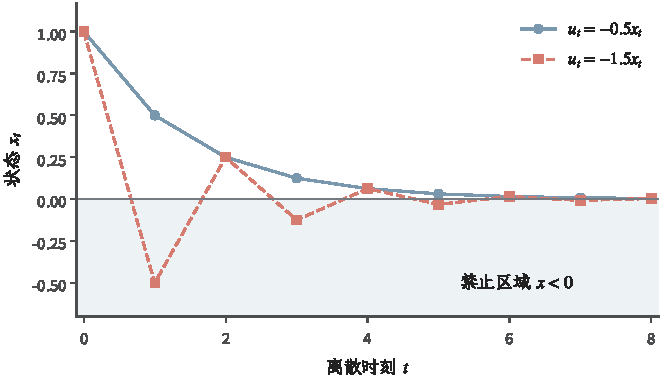
\includegraphics[width=\linewidth]{figures/math-preparation/dynamics/stability-safety.pdf}
  \caption{教学系统$x_{t+1}=x_t+u_t$从$x_0=1$出发。蓝色圆点采用$u_t=-0.5x_t$，
  保持$x_t\geq0$；红色方点采用$u_t=-1.5x_t$，第一步越过边界后交替衰减。
  两条轨迹都渐近稳定，只有前者保持安全集合$[0,\infty)$。灰色区域表示禁止的负半轴。}
  \label{fig:control-stability-safety}
\end{figure}

\subsection{控制屏障函数与可行动作}
安全函数$h$把状态是否允许转成一个标量符号，但$h$不必等于到边界的几何距离。
要判断动作会不会把状态推出集合，应观察$h$沿系统速度变化的速率。链式法则把它拆成
无控制漂移与控制引起的两部分，分别记为\term{Lie导数}（Lie derivative）：
\[
  L_{\bm{f}}h(\bm{x})
  =
  \nabla h(\bm{x})^{\top}\bm{f}(\bm{x}),
  \qquad
  L_{\bm{G}}h(\bm{x})
  =
  \nabla h(\bm{x})^{\top}\bm{G}(\bm{x}).
\]
本章把连续、严格递增、局部Lipschitz且满足$\alpha(0)=0$的函数$\alpha:\mathbb{R}\to\mathbb{R}$称为扩展类$\mathcal{K}$函数。局部Lipschitz条件保证下文标量比较系统的解局部唯一。常用选择是$\alpha(r)=\gamma r$，其中$\gamma>0$。
\begin{definition}[零化控制屏障函数]
\label{def:control-cbf}
若在某个包含$S$的开区域$D$内，对每个$\bm{x}$都有
\begin{equation}
  \sup_{\bm{u}\in U}
  \left\{
    L_{\bm{f}}h(\bm{x})
    +
    L_{\bm{G}}h(\bm{x})\bm{u}
  \right\}
  \geq
  -\alpha(h(\bm{x})),
  \label{eq:control-cbf-existence}
\end{equation}
并且上述上确界能够由某个$\bm{u}\in U$取到，则称$h$为区域$D$上的控制屏障函数（control barrier function, CBF）。
\end{definition}
这一条件及其基于二次规划的安全控制构造可参见控制屏障函数的系统论述\scite{math-ames2017cbf}
当$U$紧且花括号内的函数关于动作连续时，上确界能够取到；若这些条件不成立，只有上确界的数值不小于阈值，仍可能找不到真正满足约束的动作。定义保证每个状态至少存在一个安全动作，但实际反馈还必须从可行动作集合
\begin{equation}
  K_{\mathrm{cbf}}(\bm{x})
  =
  \left\{
    \bm{u}\in U:
    L_{\bm{f}}h(\bm{x})
    +
    L_{\bm{G}}h(\bm{x})\bm{u}
    \geq
    -\alpha(h(\bm{x}))
  \right\}
  \label{eq:control-cbf-action-set}
\end{equation}
中作出足够规则的选择。
\begin{theorem}[CBF条件保证正向不变]
\label{thm:control-cbf-invariance}
设式~\eqref{eq:control-affine-system}与式~\eqref{eq:control-safe-set}满足上述正则条件。若反馈$\bm{u}=\kappa(\bm{x})$局部Lipschitz，并对开区域$D$内每个状态满足$\kappa(\bm{x})\in K_{\mathrm{cbf}}(\bm{x})$，则$S$在相应闭环解存在的时间区间内正向不变。
\end{theorem}
\begin{proof}
沿任意闭环解令$r(t)=h(\bm{x}(t))$。链式法则与CBF约束给出
\[
  \dot r(t)
  \geq
  -\alpha(r(t)).
\]
考虑标量比较系统
\[
  \dot z(t)=-\alpha(z(t)),
  \qquad z(0)=r(0)\geq0.
\]
由于$\alpha$局部Lipschitz且$\alpha(0)=0$，标量比较系统在其最大存在区间内解唯一，$z=0$是平衡解；从非负初值出发的$z(t)$因而不能穿过零点。在闭环轨迹位于$D$且解存在的任意时间区间内，标量比较原理给出$r(t)\geq z(t)\geq0$。又因为$D$是包含$S$的开区域，轨迹若要离开$S$，必先在$D$内穿过$h=0$进入$h<0$，这与上述比较结论矛盾。因此$\bm{x}(t)\in S$在闭环解存在的全部时间内成立。

对最常用的$\alpha(r)=\gamma r$，结论可以直接验证：
\[
  \frac{\mathrm{d}}{\mathrm{d}t}
  \left(e^{\gamma t}r(t)\right)
  =
  e^{\gamma t}(\dot r(t)+\gamma r(t))
  \geq0.
\]
故$r(t)\geq e^{-\gamma t}r(0)\geq0$。边界上$r=0$时，该约束退化为$\dot r\geq0$，与式~\eqref{eq:control-nagumo-boundary}一致。
\end{proof}
该定理给出的是闭环轨迹性质，不只是某一步动作看起来朝向内部。证明依赖约束始终可行、反馈与动态具有足够正则性，以及控制信号按连续时间模型实际施加。缺少其中任一项，导数不等式都未必能沿真实轨迹成立。
\subsection{安全动作投影与二次规划}
设$\bm{u}_{\mathrm{nom}}(\bm{x})$是为性能设计的已有控制器，例如LQR反馈。可以在每个状态求解
\begin{equation}
  \begin{aligned}
    \bm{u}^{\ast}(\bm{x})
    \in\argmin_{\bm{u}\in U}\quad&
      \frac12
      (\bm{u}-\bm{u}_{\mathrm{nom}})^{\top}
      \bm{H}
      (\bm{u}-\bm{u}_{\mathrm{nom}})\\
    \text{s.t.}\quad&
      L_{\bm{f}}h(\bm{x})
      +
      L_{\bm{G}}h(\bm{x})\bm{u}
      \geq
      -\alpha(h(\bm{x})),
  \end{aligned}
  \label{eq:control-cbf-qp}
\end{equation}
其中$\bm{H}\succ\bm{0}$规定修改不同控制分量的代价。对控制仿射系统，CBF条件关于$\bm{u}$是线性不等式；若$U$是非空闭凸集，这就是具有闭凸可行域的凸二次规划。目标只表示“在该度量下尽量接近名义动作”，不表示修改后的控制仍保持原LQR成本最优。
\begin{example}[一维积分器上的安全投影]
\label{ex:control-cbf-scalar-projection}
考虑$\dot x=u$与安全集合$S=[0,\infty)$，取$h(x)=x$和$\alpha(h)=\gamma h$，其中$\gamma>0$。因为$L_fh=0$、$L_gh=1$，CBF条件正好是
\[
  u\geq-\gamma x.
\]
若$U=\mathbb{R}$、$H=1$，式~\eqref{eq:control-cbf-qp}的解是把标量名义动作投影到半直线$[-\gamma x,\infty)$：
\begin{equation}
  u^{\ast}(x)
  =
  \max\{u_{\mathrm{nom}}(x),-\gamma x\}.
  \label{eq:control-cbf-scalar-projection}
\end{equation}
例如$x=0.2$、$\gamma=1$且$u_{\mathrm{nom}}=-1$时，安全修正为$u^{\ast}=-0.2$，并使$\dot h=-h$；状态按$x(t)=0.2e^{-t}$接近边界但不穿过。若执行器还要求$u\leq-0.5$，则此状态下输入约束与CBF条件不相容，QP不可行。可行性取决于安全要求、当前状态与执行器能力的联合关系，不能由$h$的形式单独保证。
\end{example}

在$U$非空闭凸的上述条件下，若QP可行，则可行域非空且闭；正定二次目标具有强制性，因而最优解存在，严格凸性进一步保证最优动作唯一。若不要求可行域闭，严格凸性只能说明已有最优解至多一个，不能保证下确界能够取到。即使最优动作存在且唯一，也不自动意味着映射$\bm{x}\mapsto\bm{u}^{\ast}(\bm{x})$局部Lipschitz。活跃约束切换、约束梯度退化或可行域突变都可能破坏反馈正则性；要调用定理~\ref{thm:control-cbf-invariance}，还需用约束资格条件和参数化优化结果核对所选解的连续性或局部Lipschitz性质。
\begin{example}[圆形障碍外的安全修正]
\label{ex:control-cbf-obstacle}
考虑平面单积分器$\dot{\bm{p}}=\bm{u}$，要求位置留在圆形障碍外。令障碍中心为$\bm{c}$、半径为$r>0$，取
\[
  h(\bm{p})
  =
  \lVert\bm{p}-\bm{c}\rVert_2^2-r^2.
\]
安全集合是$h\geq0$。选择$\alpha(h)=\gamma h$后，CBF约束为
\begin{equation}
  2(\bm{p}-\bm{c})^{\top}\bm{u}
  \geq
  -\gamma
  \bigl(
    \lVert\bm{p}-\bm{c}\rVert_2^2-r^2
  \bigr).
  \label{eq:control-cbf-obstacle-constraint}
\end{equation}
在边界点$\bm{p}-\bm{c}=(r,0)^{\top}$处，若名义控制$\bm{u}_{\mathrm{nom}}=(-v,0)^{\top}$且$v>0$，它会直接指向障碍内部，因为左侧为$-2rv<0$。取$\bm{H}=\bm{I}$且没有其他输入约束时，二次规划把名义动作正交投影到半空间$2(\bm{p}-\bm{c})^{\top}\bm{u}\geq0$；在该边界点，修正结果为$\bm{u}^{\ast}=\bm{0}$。若名义动作还含切向分量，投影会保留切向分量，只移除指向障碍内部的法向分量。
\end{example}
多个安全条件$h_i(\bm{x})\geq0$可以产生多条线性约束，但每条单独可行不代表它们与执行器限制联合可行。两个障碍可能把系统夹在没有允许动作的位置；速度、转角或推力上限也可能阻止及时避让。加入松弛变量能够让优化器总有数值解，却同时允许违反安全约束。若这样做，松弛后的QP不再提供原来的硬不变性保证，必须明确新的故障处理或恢复区域。
图~\ref{fig:control-barrier-projection}将一维安全动作集合画在$(x,u)$平面。
对每个固定状态，可行域是一条竖直半直线；QP只需把名义动作投影到这条半直线上。
在远离边界的$x\geq1$处，名义动作$-1$本身可行；接近边界时，投影把它抬到$-x$。
动作修正由可行域决定，目标函数只规定在可行域中选择哪一个动作。

\begin{figure}[htbp]
  \centering
  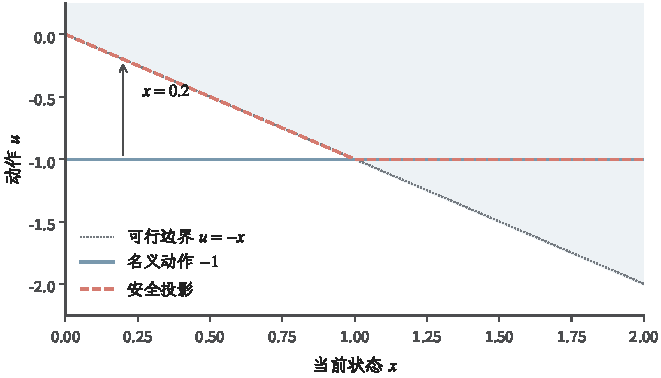
\includegraphics[width=\linewidth]{figures/math-preparation/dynamics/barrier-projection.pdf}
  \caption{教学积分器$\dot x=u$、安全集合$x\geq0$及$\alpha(h)=h$。
  灰色虚线是可行域边界$u=-x$，其上方阴影表示允许动作；蓝色实线为名义动作$u=-1$，
  红色虚线为投影$u^\star=\max\{-1,-x\}$。在$x=0.2$处，原动作修正为$-0.2$。
  此图假设无额外执行器约束，不能用来判断有限输入范围下的联合可行性。}
  \label{fig:control-barrier-projection}
\end{figure}

\subsection{鲁棒性、采样执行与高相对阶}
若真实动态含有有界加性扰动
\[
  \dot{\bm{x}}
  =
  \bm{f}(\bm{x})+\bm{G}(\bm{x})\bm{u}
  +\bm{d},
  \qquad
  \lVert\bm{d}\rVert_2\leq\delta,
\]
则最坏方向可使$\dot h$减少$\lVert\nabla h(\bm{x})\rVert_2\delta$。一个鲁棒充分条件是
\begin{equation}
  L_{\bm{f}}h
  +
  L_{\bm{G}}h\,\bm{u}
  \geq
  -\alpha(h)
  +
  \lVert\nabla h\rVert_2\delta.
  \label{eq:control-robust-cbf}
\end{equation}
模型误差也可在已有有效上界时并入类似裕量。没有经过验证的误差界时，任意加一个“安全系数”只能形成经验缓冲，不能推出鲁棒不变性。

数字控制器通常每隔$\Delta$秒求一次动作，并在两次更新之间保持不变。采样时刻满足CBF约束，不自动保证区间内部也满足，因为状态、Lie导数和最危险动作可能在区间中变化。可行做法包括用Lipschitz界为采样间变化预留裕量、直接建立离散时间屏障条件
\[
  h(\bm{x}_{t+1})-h(\bm{x}_t)
  \geq-\alpha_{\mathrm d}(h(\bm{x}_t)),
\]
其中离散比较函数应对每个$r\geq0$满足
$0\leq\alpha_{\mathrm d}(r)\leq r$。这样，只要
$h(\bm{x}_t)\geq0$，就有
\[
  h(\bm{x}_{t+1})
  \geq
  h(\bm{x}_t)-\alpha_{\mathrm d}(h(\bm{x}_t))
  \geq0,
\]
从而可以逐步归纳安全性。常用线性选择是
$\alpha_{\mathrm d}(r)=\gamma r$，其中$0<\gamma\leq1$。另一种做法是在预测时域内验证整段轨迹。连续时间证明不能省略这一实现差异。

还有一类问题来自\term{相对阶}。若$L_{\bm{G}}h(\bm{x})=\bm{0}$，控制不出现在$h$的一阶导数中，式~\eqref{eq:control-cbf-action-set}便无法限制动作。例如双积分器
\[
  \dot p=v,\qquad \dot v=u
\]
若用$h(p)=p-p_{\min}$保护位置下界，则$\dot h=v$与$u$无关，控制要到$\ddot h=u$才出现。该位置输出相对于输入具有相对阶$2$：第一次求导仍由现有速度决定，第二次才显露当前动作。
此时需使用高阶CBF，递归约束$h,\dot h$及更高导数，或把速度制动距离纳入安全函数。
例如$p-p_{\min}=0.1$、$v=-1$且最大制动加速度为$u=2$，最快停止所需距离为
$v^2/(2u)=0.25$，已经超过剩余距离。此刻即使位置仍在$S$内，也无法保证将来不越界。
这说明安全初态往往还要限制速度；只把位置约束写进一阶公式无法表达制动能力。把一阶公式机械套到$L_{\bm{G}}h=0$的情形，只会得到与控制无关的条件。

CBF还假设控制器知道用于计算$h$的状态。若只有带误差的状态估计，应对估计误差建立集合界或概率模型，再收紧安全集或构造输出反馈屏障。把估计值直接当作真实状态代入，只能证明估计轨迹满足约束，不能自动证明真实轨迹安全。
\section{用连续时间价值方程验证最优反馈}
\label{sec:control-hjb}

离散LQR与一般Bellman方程使用同一个跨时刻价值原则。
本节把时间步缩短，得到连续时间的价值方程；确定性漂移产生一阶项，扩散噪声增加二阶项。
光滑价值允许经典验证，折点与状态边界则需要更广义的解概念，并须重新核对边界条件。
\subsection{确定性HJB方程与验证定理}
有限时域LQR利用离散Bellman递推。连续时间中没有固定的一步，但可以把任意短区间$[t,t+\Delta]$视为第一步。考虑确定性受控系统
\begin{equation}
  \dot{\bm{x}}(s)
  =
  \bm{f}(\bm{x}(s),\bm{u}(s),s),
  \qquad
  \bm{x}(t)=\bm{x},
  \label{eq:control-continuous-dynamics}
\end{equation}
以及成本
\begin{equation}
  J_{t,\bm{x}}(\bm{u})
  =
  \phi(\bm{x}(T))
  +
  \int_t^T
  \ell(\bm{x}(s),\bm{u}(s),s)\,\mathrm{d}s.
  \label{eq:control-continuous-cost}
\end{equation}
价值函数为$V(\bm{x},t)=\inf_{\bm{u}}J_{t,\bm{x}}(\bm{u})$。控制$\bm{u}(s)$只能依据时刻$s$已经可用的信息；确定性完全状态反馈下，这通常表示它由当前或过去状态决定，而不能预知未来扰动。

动态规划原理把最优成本拆成短区间成本与剩余价值：
\begin{equation}
  V(\bm{x},t)
  =
  \inf_{\bm{u}|_{[t,t+\Delta]}}
  \left\{
    \int_t^{t+\Delta}
    \ell(\bm{x}(s),\bm{u}(s),s)\,\mathrm{d}s
    +
    V(\bm{x}(t+\Delta),t+\Delta)
  \right\}.
  \label{eq:control-continuous-dpp}
\end{equation}
下面给出经典形式推导。除假设$V$连续可微外，还假设动态规划原理成立，$\bm{f}$与$\ell$具有使短时轨迹偏移为$O(\Delta)$的连续性，并且短区间下确界可由可测的$\eta\Delta$-最优控制逼近，相关Taylor余项对这些控制局部一致。先在短区间内取任意常值动作$\bm{u}$。Taylor展开给出
\begin{align*}
  V(\bm{x}(t+\Delta),t+\Delta)
  &=
  V(\bm{x},t)
  +
  \Delta\,\partial_t V(\bm{x},t)\\
  &\quad+
  \Delta\,
  \nabla_{\bm{x}}V(\bm{x},t)^{\top}
  \bm{f}(\bm{x},\bm{u},t)
  +o(\Delta),
\end{align*}
而阶段积分为$\Delta\ell(\bm{x},\bm{u},t)+o(\Delta)$。由于式~\eqref{eq:control-continuous-dpp}对全部短时控制取下确界，代入这个常值动作只能先得到
\[
  -\partial_tV(\bm{x},t)
  \leq
  \ell(\bm{x},\bm{u},t)
  +
  \nabla_{\bm{x}}V(\bm{x},t)^{\top}
  \bm{f}(\bm{x},\bm{u},t).
\]
该式对每个$\bm{u}\in U$成立，故左侧不大于右侧对动作的下确界。

还需证明反向不等式。对任意$\eta>0$，在长度为$\Delta$的短区间上选择一个目标值距离下确界不超过$\eta\Delta$的允许控制。沿这条短时轨迹展开阶段成本和剩余价值，并利用每个时刻的Hamilton量都不小于其对动作的下确界，可得
\[
  \partial_tV(\bm{x},t)
  +
  \inf_{\bm{u}\in U}
  \left\{
    \ell(\bm{x},\bm{u},t)
    +
    \nabla_{\bm{x}}V(\bm{x},t)^{\top}
    \bm{f}(\bm{x},\bm{u},t)
  \right\}
  \leq
  \eta+o(1).
\]
依次令$\Delta\downarrow0$和$\eta\downarrow0$便得到反向不等式。两边合并，得到
\term{Hamilton--Jacobi--Bellman方程}：
\begin{equation}
  -\partial_tV(\bm{x},t)
  =
  \inf_{\bm{u}\in U}
  \left\{
    \ell(\bm{x},\bm{u},t)
    +
    \nabla_{\bm{x}}V(\bm{x},t)^{\top}
    \bm{f}(\bm{x},\bm{u},t)
  \right\},
  \qquad
  V(\bm{x},T)=\phi(\bm{x}).
  \label{eq:control-deterministic-hjb}
\end{equation}
花括号内的量常称为控制问题的Hamilton量，它把瞬时成本与价值沿当前速度的变化率相加，再对动作作局部优化。它不是第~\ref{chap:dynamical-systems-and-state-estimation}章Hamilton系统中沿轨迹守恒的能量函数；二者名称相近，所描述的对象和方程不同。这里采用成本最小化约定，所以写$\inf$和$-\partial_tV$；若改为奖励最大化，符号必须成套改变\scite{math-bardi1997hjb}
\begin{theorem}[确定性HJB验证定理]
\label{thm:control-hjb-verification}
设$V\in C^1$满足式~\eqref{eq:control-deterministic-hjb}及终端条件，并假设任意允许控制都产生存在到$T$的轨迹。若存在可实现反馈$\bm{u}^{\ast}=\kappa(\bm{x},t)$逐点达到HJB右侧的下确界，且相应闭环轨迹存在，则$V$等于最优价值，$\kappa$是最优反馈。
\end{theorem}
\begin{proof}
任取一个允许控制$\bm{u}(s)$及其轨迹。HJB中的下确界不大于代入该动作后的值，所以
\[
  \partial_sV(\bm{x}(s),s)
  +
  \nabla_{\bm{x}}V(\bm{x}(s),s)^{\top}
  \bm{f}(\bm{x}(s),\bm{u}(s),s)
  +
  \ell(\bm{x}(s),\bm{u}(s),s)
  \geq0.
\]
链式法则把前两项合成$\mathrm{d}V(\bm{x}(s),s)/\mathrm{d}s$。从$t$积分到$T$，并用$V(\bm{x}(T),T)=\phi(\bm{x}(T))$，得到
\[
  J_{t,\bm{x}}(\bm{u})
  \geq V(\bm{x},t).
\]
因此$V$是所有允许控制成本的共同下界。

采用$\bm{u}^{\ast}=\kappa(\bm{x},s)$时，反馈在每一点达到HJB下确界，上述不等式处处取等号。沿闭环轨迹积分便有$J_{t,\bm{x}}(\bm{u}^{\ast})=V(\bm{x},t)$。所以该反馈达到共同下界，$V$就是最优价值。
\end{proof}
HJB方程是最优性的局部必要关系；验证定理则说明一个足够光滑的候选解如何成为全局证书。仅把偏微分方程在若干采样点上的残差降得很小，还不能自动获得验证结论，因为还需终端或边界条件、可实现的极小动作、轨迹存在性以及整个相关区域上的方程关系。
\subsection{随机HJB方程与扩散生成元}
若状态服从Itô随机微分方程
\begin{equation}
  \mathrm{d}\bm{X}_s
  =
  \bm{f}(\bm{X}_s,\bm{u}_s,s)\,\mathrm{d}s
  +
  \bm{\Sigma}(\bm{X}_s,\bm{u}_s,s)\,
  \mathrm{d}\bm{W}_s,
  \label{eq:control-stochastic-dynamics}
\end{equation}
控制$\bm{u}_s$必须对当前滤过适应，不能使用未来布朗增量。价值改为期望成本的下确界。对$V\in C^{2,1}$使用第~\ref{chap:dynamical-systems-and-state-estimation}章的Itô公式，短时间条件期望中一阶随机积分均值为零，二次变差留下
\[
  \frac12
  \operatorname{tr}
  \left(
    \bm{\Sigma}\bm{\Sigma}^{\top}
    \nabla_{\bm{x}}^2V
  \right).
\]
因此随机HJB为
\begin{equation}
  \begin{aligned}
  -\partial_tV(\bm{x},t)
  =
  \inf_{\bm{u}\in U}
  \biggl\{&
    \ell(\bm{x},\bm{u},t)
    +
    \nabla_{\bm{x}}V(\bm{x},t)^{\top}
    \bm{f}(\bm{x},\bm{u},t)\\
    &+
    \frac12
    \operatorname{tr}
    \left[
      \bm{\Sigma}(\bm{x},\bm{u},t)
      \bm{\Sigma}(\bm{x},\bm{u},t)^{\top}
      \nabla_{\bm{x}}^2V(\bm{x},t)
    \right]
  \biggr\},
  \end{aligned}
  \label{eq:control-stochastic-hjb}
\end{equation}
终端条件仍为$V(\bm{x},T)=\phi(\bm{x})$。

\begin{theorem}[随机HJB验证]
\label{thm:control-stochastic-hjb-verification}
设$V$对时间一次、对状态二次连续可微，满足式~\eqref{eq:control-stochastic-hjb}及终端条件。假设每个允许的适应控制都使式~\eqref{eq:control-stochastic-dynamics}存在到$T$，成本和下述Itô各项可积，并且随机积分是真鞅。若存在可容许的反馈$\bm{u}^{\ast}=\kappa(\bm{x},t)$逐点达到HJB中的下确界，则$V$等于最优期望成本，$\kappa$是最优反馈。
\end{theorem}
\begin{proof}
记动作$\bm{u}$下的受控生成元为
\[
  \mathcal{L}^{\bm{u}}V
  =
  \nabla_{\bm{x}}V^{\top}\bm{f}
  +
  \frac12
  \operatorname{tr}
  \left(
    \bm{\Sigma}\bm{\Sigma}^{\top}
    \nabla_{\bm{x}}^2V
  \right).
\]
HJB说明，对任意允许动作都有
\[
  \partial_sV+\mathcal{L}^{\bm{u}_s}V
  +\ell(\bm{X}_s,\bm{u}_s,s)\geq0.
\]
沿受控轨迹对$V(\bm{X}_s,s)$使用Itô公式，从$t$积分到$T$并取条件期望。随机积分因真鞅条件期望为零，故
\[
  \mathbb{E}\left[
    \phi(\bm{X}_T)
    +
    \int_t^T
      \ell(\bm{X}_s,\bm{u}_s,s)\,\mathrm{d}s
    \,\middle|\,\bm{X}_t=\bm{x}
  \right]
  \geq V(\bm{x},t).
\]
所以$V$是所有允许控制期望成本的下界。对反馈$\kappa$，HJB下确界逐点达到，上述生成元不等式取等号；重复同一计算便得到其期望成本恰为$V(\bm{x},t)$，从而完成验证。
\end{proof}
若随机积分只是局部鞅，直接断言其期望为零可能失败；通常需要增长界、停时局部化与一致可积性等条件把局部结论提升为上述等式。随机HJB的局部形式本身不能替代这些可积性检查。

若扩散矩阵与动作无关，且价值是二次函数，二阶项可能只增加与状态无关的常数，这与离散LQR中式~\eqref{eq:control-lqr-noise-constant}的现象一致。若$\bm{\Sigma}$依赖动作或状态，二阶项会参与动作最小化或改变价值的状态形状，反馈一般也会改变。
\subsection{连续时间LQR与微分Riccati方程}
用HJB重新考察线性二次问题。令
\[
  \dot{\bm{x}}
  =
  \bm{A}\bm{x}+\bm{B}\bm{u},
\]
阶段成本和终端成本分别为
\[
  \ell(\bm{x},\bm{u})
  =
  \bm{x}^{\top}\bm{Q}\bm{x}
  +
  \bm{u}^{\top}\bm{R}\bm{u},
  \qquad
  \phi(\bm{x})
  =
  \bm{x}^{\top}\bm{Q}_T\bm{x},
\]
其中$\bm{Q},\bm{Q}_T\succeq\bm{0}$、$\bm{R}\succ\bm{0}$。设
\[
  V(\bm{x},t)
  =
  \bm{x}^{\top}\bm{P}(t)\bm{x},
  \qquad
  \bm{P}(T)=\bm{Q}_T,
\]
并取$\bm{P}(t)$对称。于是
\[
  \partial_tV
  =
  \bm{x}^{\top}\dot{\bm{P}}(t)\bm{x},
  \qquad
  \nabla_{\bm{x}}V
  =
  2\bm{P}(t)\bm{x}.
\]
代入确定性HJB，动作相关项为
\[
  \bm{u}^{\top}\bm{R}\bm{u}
  +
  2\bm{x}^{\top}\bm{P}\bm{B}\bm{u}.
\]
同样配方：
\begin{align*}
  &\bm{u}^{\top}\bm{R}\bm{u}
  +
  2\bm{x}^{\top}\bm{P}\bm{B}\bm{u}\\
  &\quad=
  \left(
    \bm{u}+\bm{R}^{-1}\bm{B}^{\top}\bm{P}\bm{x}
  \right)^{\top}
  \bm{R}
  \left(
    \bm{u}+\bm{R}^{-1}\bm{B}^{\top}\bm{P}\bm{x}
  \right)
  -
  \bm{x}^{\top}
  \bm{P}\bm{B}\bm{R}^{-1}\bm{B}^{\top}\bm{P}
  \bm{x}.
\end{align*}
所以最优反馈为
\begin{equation}
  \bm{u}^{\ast}(t)
  =
  -\bm{R}^{-1}\bm{B}^{\top}\bm{P}(t)\bm{x}(t),
  \label{eq:control-continuous-lqr-gain}
\end{equation}
而对任意$\bm{x}$比较二次型系数，得到
\begin{equation}
  -\dot{\bm{P}}
  =
  \bm{Q}
  +
  \bm{A}^{\top}\bm{P}
  +
  \bm{P}\bm{A}
  -
  \bm{P}\bm{B}\bm{R}^{-1}\bm{B}^{\top}\bm{P},
  \qquad
  \bm{P}(T)=\bm{Q}_T.
  \label{eq:control-continuous-riccati}
\end{equation}
这就是连续时间微分Riccati方程。它从终端条件向较早时刻反向积分；式中的负号反映价值边界给在终点，而不是数值积分器可以任意忽略的记号。

无限时域稳态令$\dot{\bm{P}}=\bm{0}$，得到连续代数Riccati方程
\begin{equation}
  \bm{0}
  =
  \bm{Q}
  +
  \bm{A}^{\top}\bm{P}
  +
  \bm{P}\bm{A}
  -
  \bm{P}\bm{B}\bm{R}^{-1}\bm{B}^{\top}\bm{P}.
  \label{eq:control-care}
\end{equation}
此时稳定的含义改为闭环矩阵$\bm{A}-\bm{B}\bm{R}^{-1}\bm{B}^{\top}\bm{P}$的全部特征值实部为负。在连续时间版本的可稳定、可检测条件下，选取半正定稳定化解可得到无限时域最优反馈。离散DARE和连续CARE外形相近，却分别对应单位圆和左半平面的稳定区域，不能混用。
\subsection{非光滑价值、边界条件与部分观测}
经典HJB推导假设价值足够光滑，但最优控制常产生切换面、状态约束或不可微终端成本。
此时价值可能连续，却没有处处可用的梯度或Hessian矩阵。困难在于方程含有导数，不能
把一个折点直接代入经典公式。\term{黏性解}（viscosity solution）用光滑函数从上下两侧
接触价值，在接触点检验方程的不等式；导数取自接触函数，价值本身可以没有导数。

为固定不等式方向，将前面的确定性HJB写成
\[
  F(\bm x,t,a,\bm p)
  :=-a-\inf_{\bm u\in U}\{\ell(\bm x,\bm u,t)
                       +\bm p^\top\bm f(\bm x,\bm u,t)\}=0,
\]
其中$a$和$\bm p$分别代表时间导数与状态梯度。
\begin{definition}[连续价值函数的黏性解]
  \label{def:control-viscosity-solution}
  设$V$在HJB作用域内连续。若对任意光滑测试函数$\varphi$，当$V-\varphi$在
  内点$(\bm x,t)$取得局部最大值时，都有
  $F(\bm x,t,\partial_t\varphi,\nabla\varphi)\leq0$，称$V$为黏性次解。
  若局部最小值处都满足相应的$F\geq0$，称为黏性上解。
  同时满足两项，且按当前问题满足终端或边界条件的$V$，称为黏性解。
\end{definition}
测试函数可平移一个常数，使接触时$V=\varphi$。局部最大意味着测试函数在邻域内
位于价值上方并与之接触，局部最小则对应位于价值下方的接触；测试函数的导数必须
符合这个局部接触条件。
随机二阶HJB还要把测试函数的Hessian代入$F$。当$V$足够光滑时，取$\varphi=V$
便同时得到$F\leq0$与$F\geq0$，恢复经典等式。在适当函数类和边界条件下，比较原理
使每个次解不高于每个上解，从而给出唯一性；比较原理本身仍有连续性、增长与方程结构
条件，不能由这个定义自动推出。

一维最短到达问题说明为什么必须先区分延续域与目标边界。令$\dot x=u$、$|u|\leq1$，每经过一单位时间支付成本$1$，到达目标集合$\{0\}$时终止。最短到达时间是
\[
  V(x)=|x|.
\]
在$x\neq0$处，稳态HJB为
\[
  0
  =
  1+\inf_{|u|\leq1}V'(x)u
  =
  1-|V'(x)|,
\]
最优控制分别取$u=-1$和$u=1$，把左右两侧的状态推向原点。价值在$x=0$处没有经典导数，但$x=0$是退出目标边界，不属于延续域$\mathbb{R}\setminus\{0\}$；HJB在两个延续分支上都由经典导数满足，目标点只需施加$V(0)=0$的边界条件。因此，这个例子说明全局价值可以在目标边界非光滑，却不能单独证明延续域内部必须使用黏性解。只有当切换面、状态约束或非光滑终端数据使折点落在方程作用域内时，才需要用上方或下方的光滑测试函数解释该点的HJB不等式；相应唯一性仍依赖当前边界条件、函数增长类和Hamilton量的比较原理。

\begin{example}[延续域内部的价值折点]
  \label{ex:control-viscosity-interior-kink}
  仍取$\dot x=u$、$|u|\leq1$，但不在到达原点时退出：固定终点$T$，运行成本为零，
  终端成本为$|x(T)|$。从$(x,t)$出发最多移动$T-t$的距离，因此
  \[
    V(x,t)=\max\{|x|-(T-t),0\}.
  \]
  在$|x|<T-t$时可以到达原点并停留，价值为零；在外侧，剩余时间只能减去$T-t$
  的距离。HJB为$-V_t+|V_x|=0$，终端条件为$V(x,T)=|x|$。
  折点$x=\pm(T-t)$位于延续域内部，经典导数在这里不存在。
  例如$T-t=1$时，$|x|\leq1$都能在终点前到达原点，价值为零；$x=1.5$的最低终端代价为$0.5$。
  $x=1$处的折角因此分开“时间足够完全纠正”和“仍有不可消除终端偏差”两类状态。

  以正侧折点为例，局部价值为$\max\{x+t-T,0\}$。从下方接触的光滑函数在接触点
  的导数对$(\varphi_x,\varphi_t)$属于$(p,p)$、$0\leq p\leq1$，对应两侧斜率的
  凸组合。因此$-\varphi_t+|\varphi_x|=-p+p=0$，满足上解条件。
  空间方向的向上折角使该点没有光滑的上方接触函数，次解检验在这里没有额外约束；
  光滑区域则由经典等式同时满足两项条件。负侧同理。
  这个可直接求出最优成本的例子说明，黏性条件确实能在方程作用域内部处理折点，
  而不需要把切换面误当作终止边界。
\end{example}

状态约束也需要边界条件。若边界不可穿越，价值只在可行控制存在的区域定义，HJB必须与可行方向或状态约束边界条件共同解释。若允许碰到边界后终止，则应给出退出成本。仅在区域内部求出一个光滑解，不能决定边界上的控制含义。

当真实状态不可见时，把$\bm{x}$直接作为HJB状态也不可实现。一般做法是把给定观测历史的条件状态分布作为\term{信念状态}；它包含当前决策所需的信息，但通常是无限维对象。线性高斯二次问题具有特殊的分离结构，可以用Kalman估计配合LQR反馈；一般部分观测、风险敏感或受约束问题则不能从分离原理直接推出最优性。

HJB、LQR和CBF之间也有清楚边界。HJB寻找指定成本下的最优反馈，CBF把安全性写成每个状态的动作可行约束。可以在HJB中加入状态约束，也可以用CBF-QP修正性能控制器，但前者需要求解受约束动态优化，后者通常牺牲原性能最优性。稳定价值函数、最优价值函数和屏障函数都沿轨迹考察标量变化，却分别证明收敛、最优和不变性，不能只因公式都含导数就互相替代。
\section{本章小结}
\label{sec:control-theory-summary}

控制把给定输入下的状态演化改成闭环选择问题。在线性系统中，可控性要求输入能够生成全部状态方向，可稳定性只要求输入能够改变不稳定模式；可观测性要求输出区分全部初态，可检测性只要求不可见模式自行稳定。秩判据给出有限时域的整体检查，PBH判据直接定位危险特征模式。可稳定与可检测共同支持观测器和状态反馈的分离设计，但这个结论依赖线性结构及相应信息条件。

有限时域LQR把线性动态、二次成本和Bellman递推闭合在二次价值函数族中。逐步配方给出线性反馈增益与Riccati反向递推；零均值独立加性噪声只增加价值常数项。本章的无折扣无限时域LQR改用确定性系统：它不能接受任意代数Riccati根，而要在可稳定、可检测及代价正定条件下选择半正定稳定化解。滤波Riccati与控制Riccati具有矩阵对偶结构；在标准线性高斯条件下，条件状态均值可以接入LQR反馈而保持期望成本最优，但信息、噪声或约束改变后必须重新验证分离。

成本最优不等于安全。正向不变性要求每条闭环轨迹持续留在允许集合内；CBF将边界方向条件扩展为集合附近的动作不等式，并可通过二次规划最小修改名义控制器。该保证以动作约束可行、反馈正则、状态信息可靠和连续模型与实际执行一致为前提。扰动、模型误差、采样保持、输入上限和高相对阶都会改变需要验证的条件。

连续时间Bellman原理在短时间极限下产生HJB方程；随机动态借助Itô公式多出扩散的二阶项。验证定理把HJB解、达到极小值的反馈和全时域最优性连接起来，连续时间LQR则把这一关系化为微分与代数Riccati方程。价值在HJB作用域内非光滑时需要黏性解等广义概念，目标边界上的非光滑则要与边界条件一同解释；部分观测需要信念状态或具有专门分离结构的估计器。由此可以区分本章的三类保证：稳定性控制长期衰减，最优性比较累计成本，安全性保持允许集合；完整的受控系统往往需要同时核对三者。

第~\ref{chap:game-theory-and-multi-agent-decision}章将放开“环境规律与其他参与者策略固定”
这一前提，研究多方同时调整行动时的响应、均衡与学习保证。
